

\tikzset{every picture/.style={line width=0.75pt}} %set default line width to 0.75pt        

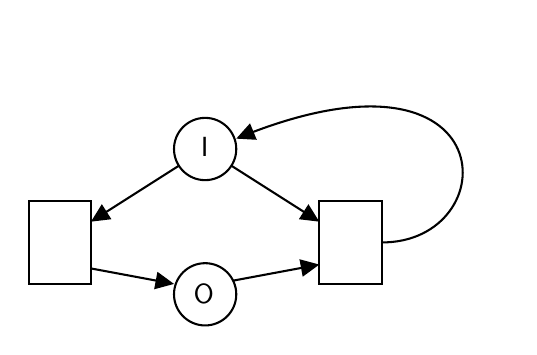
\begin{tikzpicture}[x=0.75pt,y=0.75pt,yscale=-1,xscale=1]
%uncomment if require: \path (0,142); %set diagram left start at 0, and has height of 142

%Straight Lines [id:da45933977980943075] 
\draw    (130,110) -- (177.05,101.23) ;
\draw [shift={(180,100.68)}, rotate = 529.44] [fill={rgb, 255:red, 0; green, 0; blue, 0 }  ][line width=0.08]  [draw opacity=0] (8.93,-4.29) -- (0,0) -- (8.93,4.29) -- cycle    ;
%Straight Lines [id:da664463868690055] 
\draw    (60,100.68) -- (107.05,109.45) ;
\draw [shift={(110,110)}, rotate = 190.56] [fill={rgb, 255:red, 0; green, 0; blue, 0 }  ][line width=0.08]  [draw opacity=0] (8.93,-4.29) -- (0,0) -- (8.93,4.29) -- cycle    ;
%Straight Lines [id:da3574578184910957] 
\draw    (125,45) -- (177.47,78.39) ;
\draw [shift={(180,80)}, rotate = 212.47] [fill={rgb, 255:red, 0; green, 0; blue, 0 }  ][line width=0.08]  [draw opacity=0] (8.93,-4.29) -- (0,0) -- (8.93,4.29) -- cycle    ;
%Shape: Rectangle [id:dp6093756470807308] 
\draw  [fill={rgb, 255:red, 255; green, 255; blue, 255 }  ,fill opacity=1 ] (40,70) -- (70,70) -- (70,110) -- (40,110) -- cycle ;
%Straight Lines [id:da4792886661318454] 
\draw    (125,45) -- (72.53,78.39) ;
\draw [shift={(70,80)}, rotate = 327.53] [fill={rgb, 255:red, 0; green, 0; blue, 0 }  ][line width=0.08]  [draw opacity=0] (8.93,-4.29) -- (0,0) -- (8.93,4.29) -- cycle    ;
%Shape: Circle [id:dp1215746373296942] 
\draw  [fill={rgb, 255:red, 255; green, 255; blue, 255 }  ,fill opacity=1 ] (110,45) .. controls (110,36.72) and (116.72,30) .. (125,30) .. controls (133.28,30) and (140,36.72) .. (140,45) .. controls (140,53.28) and (133.28,60) .. (125,60) .. controls (116.72,60) and (110,53.28) .. (110,45) -- cycle ;
%Shape: Rectangle [id:dp3355669008063715] 
\draw  [fill={rgb, 255:red, 255; green, 255; blue, 255 }  ,fill opacity=1 ] (180,70) -- (210,70) -- (210,110) -- (180,110) -- cycle ;
%Curve Lines [id:da5662597241143124] 
\draw    (210,90) .. controls (270.06,90.4) and (270.75,-12.96) .. (141.95,39.2) ;
\draw [shift={(140,40)}, rotate = 337.56] [fill={rgb, 255:red, 0; green, 0; blue, 0 }  ][line width=0.08]  [draw opacity=0] (8.93,-4.29) -- (0,0) -- (8.93,4.29) -- cycle    ;
%Shape: Circle [id:dp5814166449818703] 
\draw  [fill={rgb, 255:red, 255; green, 255; blue, 255 }  ,fill opacity=1 ] (110,115) .. controls (110,106.72) and (116.72,100) .. (125,100) .. controls (133.28,100) and (140,106.72) .. (140,115) .. controls (140,123.28) and (133.28,130) .. (125,130) .. controls (116.72,130) and (110,123.28) .. (110,115) -- cycle ;

% Text Node
\draw (121.5,38) node [anchor=north west][inner sep=0.75pt]   [align=left] {$\mathsf{I}$};
% Text Node
\draw (118,108.5) node [anchor=north west][inner sep=0.75pt]   [align=left] {$\mathsf{O}$};


\end{tikzpicture}